\chapter{Evaluierung}

\section{Benutzerevaluierung}
\paragraph{}
Damit es festgestellt werden könnte, ob die Anreicherung von Suchergebnissen mit aus den Snippets extrahierten Entitäten für den Benutzer auch tatsächlich hilfreich sein könnte, wurde eine Benutzerevaluierung durchgeführt. Die Evaluierung sollte folgende Fragen beantworten:

\begin{itemize}
\item Welcher Einsatz liefert dem Benutzer die zu der Anfrage am besten passende Entitäten? 
\item Wird die Geschwindigkeit der Suche durch zusätzlicher Schritt der Extraktion von Entitäten stark beeinträchtigt? Ist die Beeinträchtigung der Geschwindigkeit groß Genug, um den Benutzer bei der Suche zu stören?
\item Gibt es Korrelationen zwischen ,,standarten`` Metriken wie F-Measure und Precision/Recall und der Zufriedenheit der Benutzer, oder kann man aus der rein numerischen Metriken keine Aussage treffen, ob der Engine in der Lage ist, eine genügende Benutzerunterstützung zu leisten?
\end{itemize}

Um diese Fragen beantworten zu können, wurde eine Webseite aufgebaut, die dem Benutzer die Möglichkeit gibt, alle Engines und alle Modellen, die im Rahmen dieser Arbeit verwendet wurden, zu bewerten. Insgesamt kann der Evaluirungsvorgang in drei Schritten geteilt werden:

\begin{enumerate}
\item In dem Einleitungsschritt wird dem Benutzer erklärt, wie genau die Evaluierung abläuft, und was wir von ihm brauchen.
\item Danach muss der Benutzer alle vorhandene Kombinationen von Modellen und Engines bewerten. Dazu soll eine Frage aus der vorgegebenen Liste ausgewählt und gestellt werden, die zuerst an Bing gesendet wird, und dann an unseres Stanbol-Backend.
\item Um die Situation, wo der Benutzer sich ,,betrogen`` fühlen könnte, möglichst auszuschließen, wird dem Probanden die Möglichkeit gegeben, jede beliebige Frage zu stellen, und dann einen persönlichen schriftlichen Feedback abzugeben.
\end{enumerate}

\begin{figure}
\centering
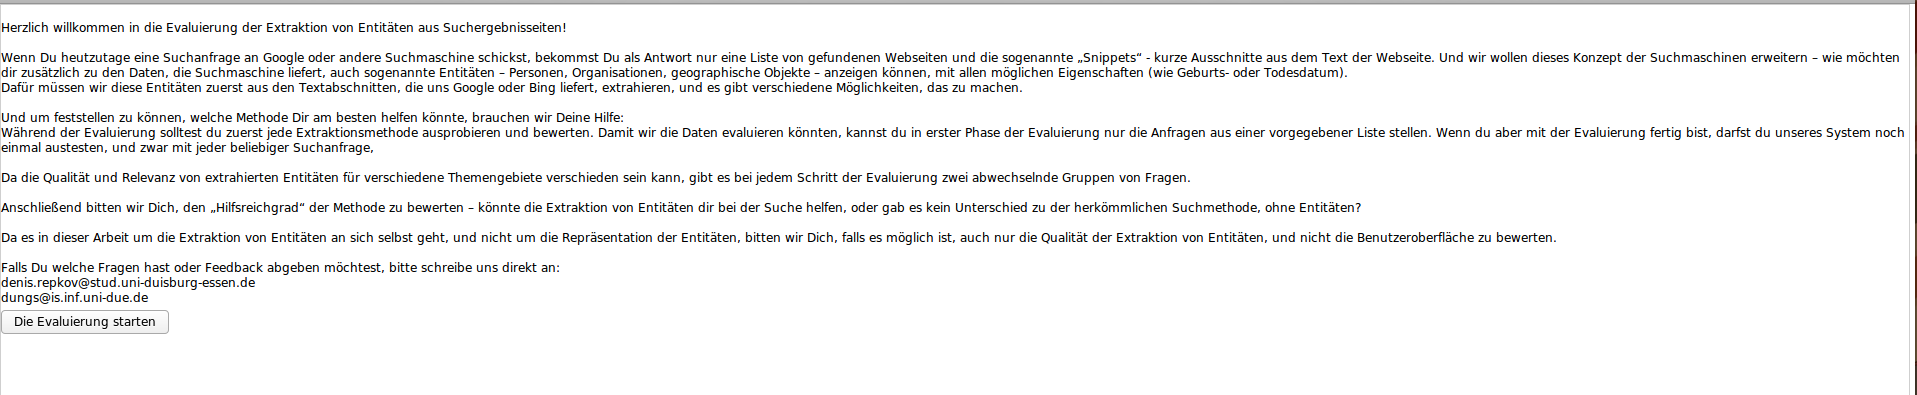
\includegraphics[width=1.0\textwidth]{Bilder/evalstep1.png}
\caption{''Einleitung in die Evaluierung''}
\label{fig:evalstep01}
\end{figure}

\begin{figure}
\centering
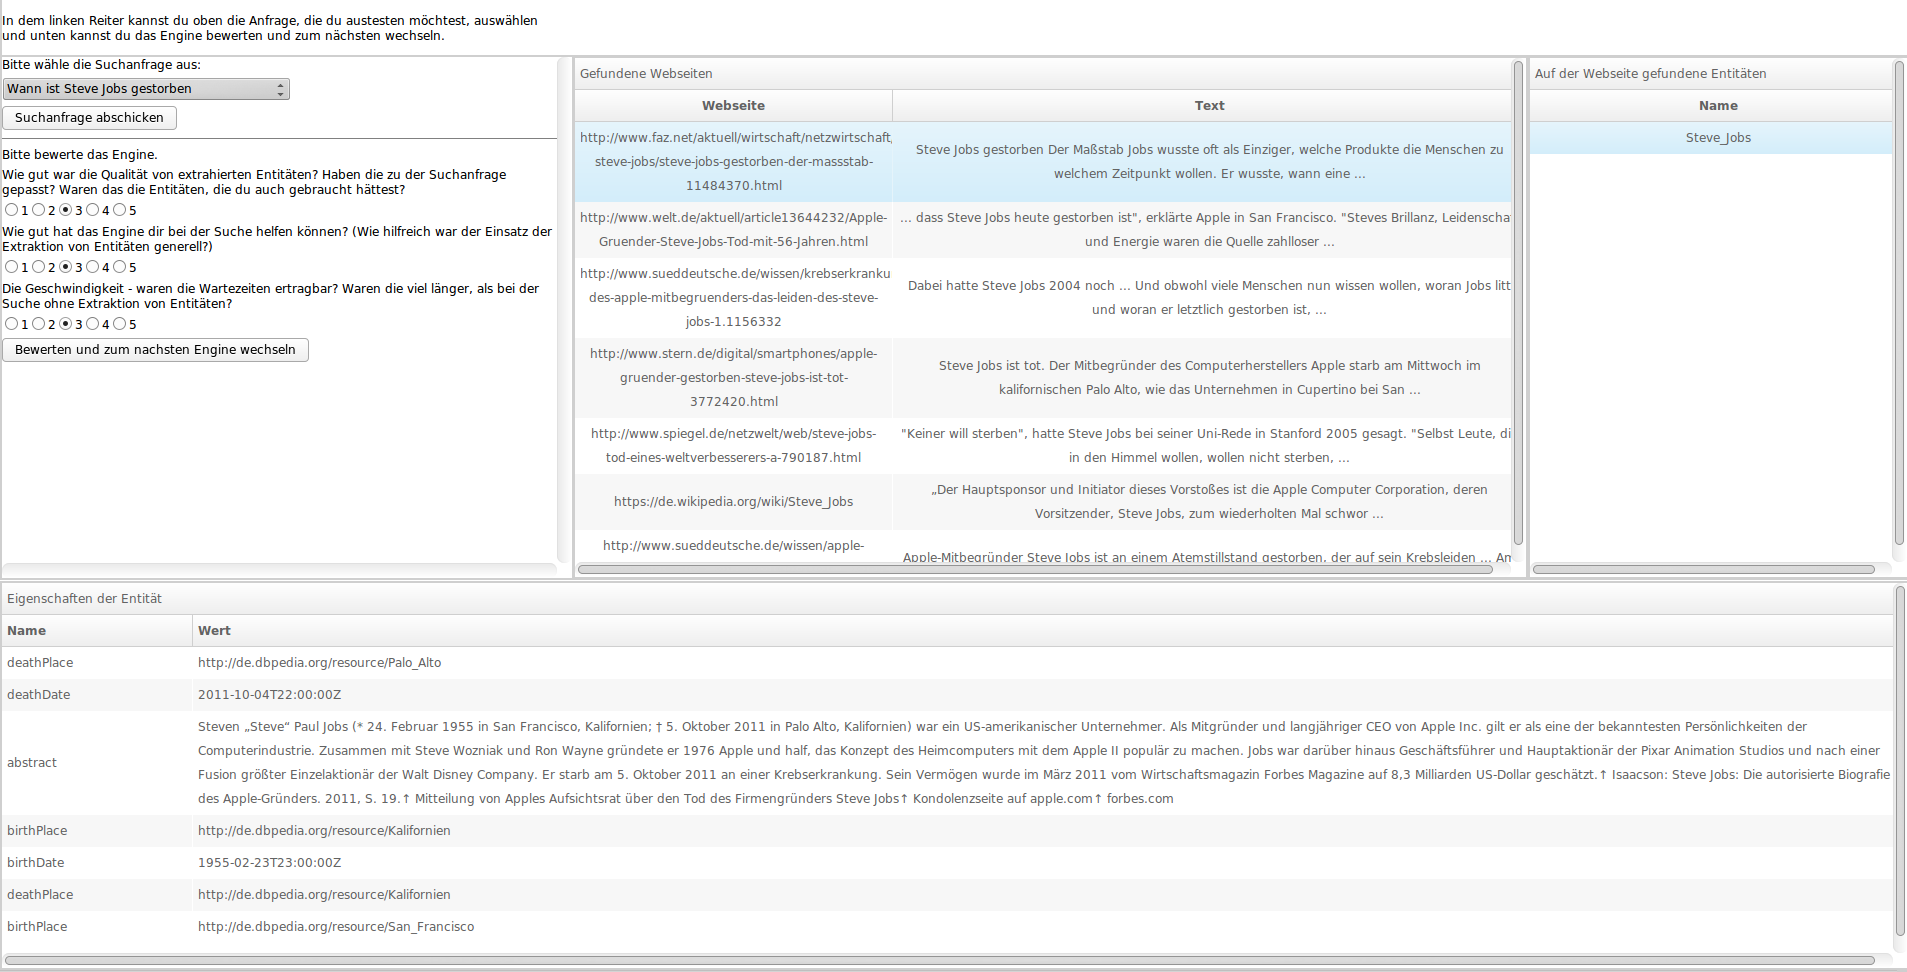
\includegraphics[width=1.0\textwidth]{Bilder/evalstep2.png}
\caption{''Bewertung eines Engines''}
\label{fig:evalstep01}
\end{figure}

\begin{figure}
\centering
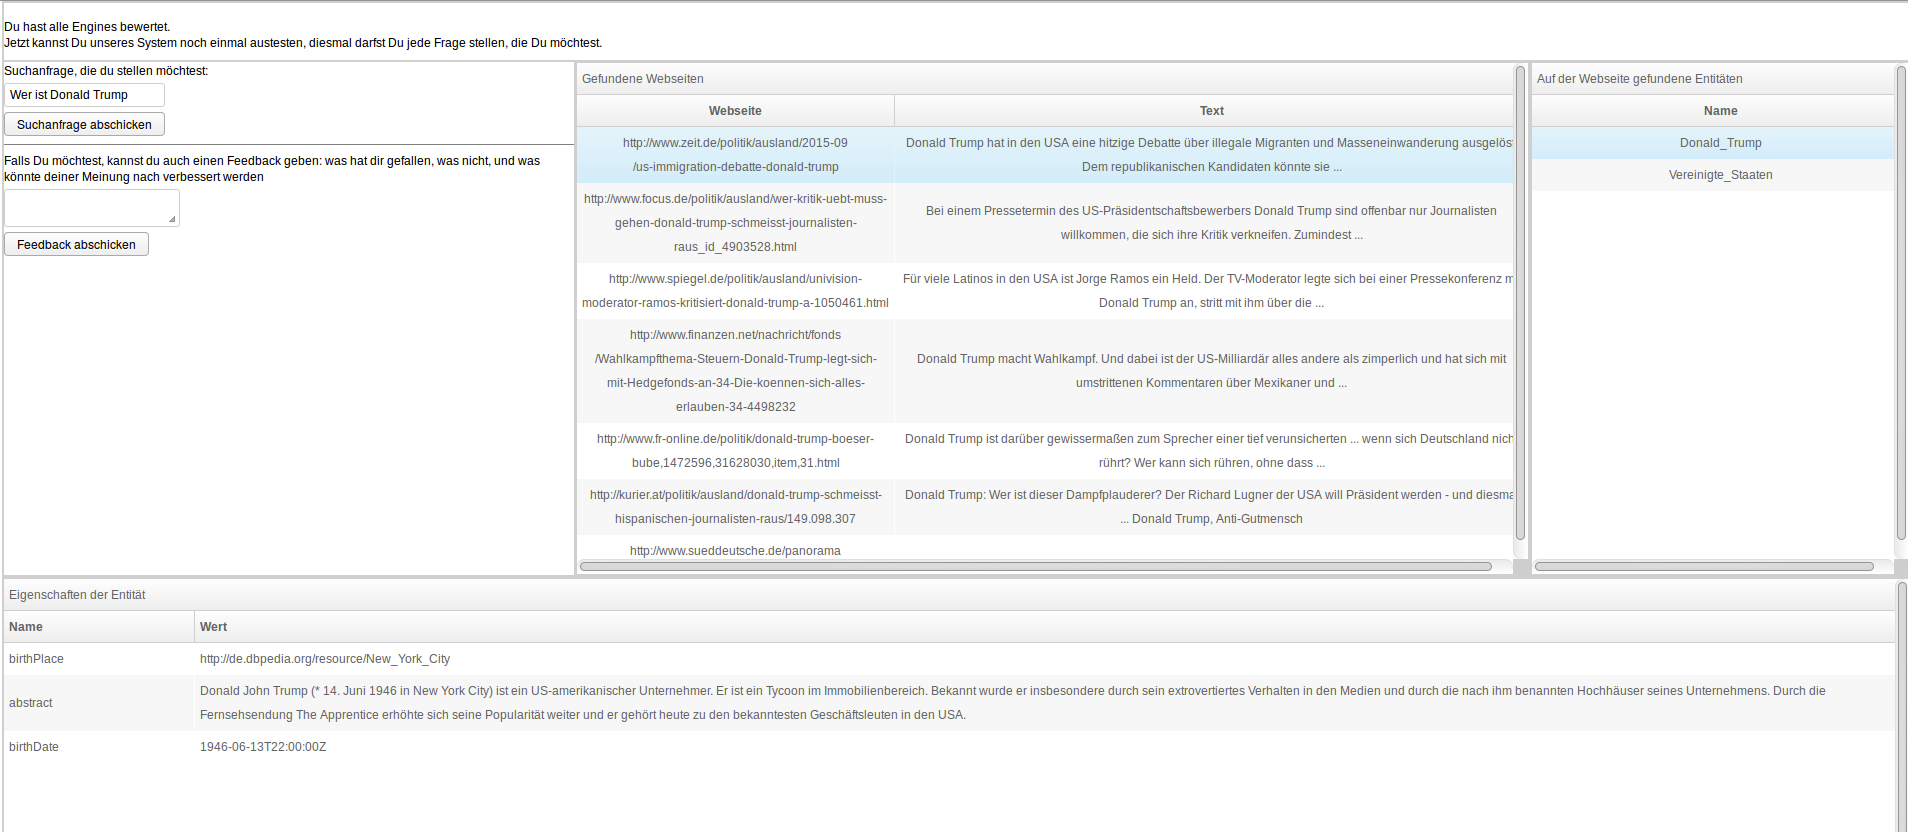
\includegraphics[width=1.0\textwidth]{Bilder/evalstep3.png}
\caption{''Der letzte Schritt der Evaluierung''}
\label{fig:evalstep01}
\end{figure}

Für jedes Engine sollen insgesamt drei Charakteristiken bewertet werden:
\begin{enumerate}
\item Qualität von extrahierten Entitäten - der Benutzer soll beschreiben, wie gut seiner Meinung nach die Entitäten zu den extrahierten Snippets gepasst haben, ob diese ,,korrekt`` von dem Gesichtspunkt des Probanden waren, ob es für die gefundene Entitäten die Daten vorhanden sind, die der Benutzer auch wirklich braucht, und ob es die Informationen gibt, die für die Suche eigentlich kaum zu Nutzen sind.
\item Geschwindigkeit der Anreicherung - Der Proband soll angeben, ob die die Extraktion von Entitäten mit der Suche zusammen schnell genug waren, besonders im Vergleich zu den Suchmaschinen wie Google oder Bing.
\item ,,Hilfreichsgrad`` von dem Ansatz - Damit soll der Benutzer uns mitteilen, ob solch eine Anreicherung von herkömmlichen Suchergebnissen mit den Entitäten und dazugehörigen Informationen wie Geburtstag/Geburtsort/u.s.w. für die Präzision der Suchanfrage hilfreich wäre, und ob der Proband den Einsatz dieser Suchmethode sinnvoll fände.  
\end{enumerate}

\subsection{Analyse der Ergebnissen}
\paragraph{}
Während der Studie wurden insgesamt 44 Bewertungen gesammelt, deren Ergebnisse in der Tabelle \ref{table:RESULTS} zu sehen sind. Es wurden außerdem einige Feedbacks gesammelt, die für die Analyse der Arbeit und als Quelle für Verbesserungsvorschläge verwendet werden können. Die Liste von Feedbacks findet man in der Auflistung \ref{lst:feedbacks}. Aber welche Schlussfolgerungen lassen sich daraus ziehen? Auf dem ersten Blick fallen folgende Besonderheiten auf:
\begin{itemize}
\item Die Benutzer fanden den Einsatz hilfreich, wünschen sich aber die Verbesserung von dem Benutzerinterface des Systems.
\item Es werden eventuell zu viel Informationen angezeigt, so dass der Benutzer sich verwirrt fühlen könnte.
\end{itemize}

\section{Automatisierte Evaluierung von Qualität der Extraktion}
\paragraph{}
Es stellt sich allerdings die Frage, ob die aus der Benutzerstudie gewonnene Ergebnisse mit den in natürsprachlicher Mensch-Computer-Interaktion übliche Evaluierungsmethoden wie 
\begin{itemize}
\item Präzision
\item Recall
\item F-Measure
\end{itemize}
vereinbart werden könnten? Was ist für den Benutzer wichtige - dass das Engine so wenig False-Positiv-Treffer wie möglich liefert, oder ob die FP für den Benutzer ehe keine bedeutende Rolle spielen? Kann man anhand statistischen Messdaten sagen können, ob das Engine auch aus Sicht des Benutzers positiv oder negativ bewertet wird? Um diese Fragen beantworten zu können, müssen noch statistische Messungen durchgeführt werden und ihre Ergebnisse mit den aus der Benutzerevaluierung gewonnenen Daten vergleichen.

\section{Vergleich zwischen Benutzer- und Datenevaluierung}
Erkenntnissen aus der Studie und den Konsequenzen für die Arbeit.